\documentclass[runningheads]{llncs}
\usepackage{graphicx}
\usepackage{amsmath}
\usepackage{booktabs}
\usepackage{hyperref}
\usepackage{multirow}
\usepackage{listings}
\usepackage{float}

\begin{document}

\title{English to Urdu Neural Machine Translation \\ using a Vanilla RNN Encoder-Decoder Architecture}
\author{First Author \and Second Author}
\institute{University/Institution Name \\ \email{\{author1, author2\}@example.com}}

\maketitle

\begin{abstract}
This report details the design, implementation, and evaluation of a Neural Machine Translation (NMT) system strictly utilizing a Vanilla Recurrent Neural Network (RNN) architecture. The objective is to translate English sentences into Urdu using a parallel corpus of approximately 9,103 pairs. We cover the full pipeline: data preprocessing, sequence encoding, dynamic batching, model training, hyperparameter tuning, and decoding (Greedy vs. Beam Search). We establish a deterministically reproducible framework, achieving a Greedy BLEU-1 score of 9.746 without utilizing attention mechanisms or advanced gating (LSTM/GRU). We conclude with a comprehensive qualitative error analysis discussing the significant limitations inherent to Vanilla RNN architectures in handling long-range structural reordering between SVO (English) and SOV (Urdu) languages.

\keywords{Neural Machine Translation \and Vanilla RNN \and Seq2Seq \and English-Urdu \and Low-Resource Translation}
\end{abstract}

\section{Introduction}
Machine Translation (MT) for morphologically rich and structurally distinct language pairs such as English (Subject-Verb-Object) and Urdu (Subject-Object-Verb) presents a notable challenge. This study implements an English-to-Urdu NMT system using a simple Vanilla RNN Encoder-Decoder architecture, adhering to constraints that prohibit long short-term memory (LSTM), gated recurrent units (GRU), or attention mechanisms. This report documents the systematic approach from data ingestion to qualitative evaluation.

\begin{figure}[H]
    \centering
    
\includegraphics[width=\textwidth]{outputs/plots/11_final_dashboard.png}
    \caption{Final Project Evaluation Dashboard Summary}
    \label{fig:dashboard}
\end{figure}

\section{Data Preprocessing and Splitting}

\subsection{Data Cleaning and Normalization}
The original Kaggle English-to-Urdu dataset comprises 9,103 parallel sentences. Distinct pipelines were developed for both source and target languages:
\begin{itemize}
    \item \textbf{English:} Lowercasing, Unicode NFKC normalization, URL/email stripping, and regex-based punctuation clearing.
    \item \textbf{Urdu:} Removal of zero-width non-joiners (ZWNJ), Urdu-specific regex mapping, and punctuation normalization (e.g., converting standard commas to Urdu commas).
\end{itemize}

\begin{figure}[H]
    \centering
    
\includegraphics[width=0.8\textwidth]{outputs/plots/01_corpus_exploration.png}
    \caption{Initial Corpus Exploration and Statistics}
    \label{fig:corpus}
\end{figure}

Quality filtering was subsequently applied. Sentence pairs containing empty sequences or exhibiting extreme length ratios ($<0.3$ or $>3.0$) were dropped. Post-cleaning, 8,542 legitimate pairs were retained.

\begin{figure}[H]
    \centering
    
\includegraphics[width=0.8\textwidth]{outputs/plots/02_preprocessing_analysis.png}
    \caption{Preprocessing and Sentence Length Distribution Analysis}
    \label{fig:preprocessing}
\end{figure}

\subsection{Train-Validation-Test Split}
To guarantee zero data leakage, we grouped the dataset by unique English source sentences before employing a stratified split. Using a fixed random seed (\texttt{SEED=42}), the data generated the following non-overlapping splits:
\begin{itemize}
    \item \textbf{Training Set:} 6,823 samples ($\sim$80\%)
    \item \textbf{Validation Set:} 864 samples ($\sim$10\%)
    \item \textbf{Test Set:} 855 samples ($\sim$10\%)
\end{itemize}

\begin{figure}[H]
    \centering
    
\includegraphics[width=0.6\textwidth]{outputs/plots/03_dataset_split.png}
    \caption{Train-Validation-Test Dataset Split Proportions}
    \label{fig:split}
\end{figure}

\section{Tokenization and Sequence Processing}

\subsection{Vocabulary Construction}
Word-level tokenization was implemented. A custom \texttt{Vocabulary} class was constructed dynamically utilizing solely the training set to prevent leakage. We established four special tokens: \texttt{<pad>}, \texttt{<bos>}, \texttt{<eos>}, and \texttt{<unk>}. A minimum token frequency threshold of 2 was applied; words falling below this threshold were mapped to \texttt{<unk>}. 

\begin{table}[H]
    \centering
    \caption{Vocabulary Dimensions Post-Filtering}
    \begin{tabular}{lc}
        \toprule
        \textbf{Property} & \textbf{Value} \\
        \midrule
        English Vocabulary Size & 3,821 \\
        Urdu Vocabulary Size & 4,094 \\
        Min Token Frequency & 2 \\
        \bottomrule
    \end{tabular}
\end{table}

\begin{figure}[H]
    \centering
    
\includegraphics[width=0.8\textwidth]{outputs/plots/04_vocabulary_analysis.png}
    \caption{Vocabulary Dimensions and Word Frequencies}
    \label{fig:vocab}
\end{figure}

\subsection{Masking, Padding, and Batching}
The integer-encoded sequences were seamlessly combined using a custom collate function. Instead of padding every sentence to a global maximum length, we implemented \textbf{dynamic padding}, wherein sequences are only padded to the maximum length of their respective batch. This approach significantly minimizes computational waste during the forward pass. Teacher forcing inputs (decoder inputs) and shifted target outputs were generated directly within this pipeline.

\begin{figure}[H]
    \centering
    
\includegraphics[width=0.8\textwidth]{outputs/plots/05_batch_structure.png}
    \caption{Dynamic Padding and Batch Structure Visualization}
    \label{fig:batching}
\end{figure}

\section{Model Architecture}
The Encoder-Decoder framework is constructed exclusively via \texttt{torch.nn.RNN} layers utilizing \texttt{tanh} activations.

\subsection{Vanilla RNN Encoder}
The encoder processes the embedded source sequence chronologically. Because there is no attention mechanism, the entire syntactic and semantic meaning of the source sentence is forcefully compressed into the final hidden state, $h_T$, known as the \textbf{Context Vector}.

\subsection{Vanilla RNN Decoder}
The decoder is initialized with $h_T$. During training, it leverages \textbf{Teacher Forcing} to stabilize the learning gradients. The decoder output is projected via a linear layer across the target vocabulary, and cross-entropy loss is computed against the shifted target sequence. \textbf{Label Smoothing} ($\epsilon=0.1$) is utilized to penalize overconfidence.

\begin{figure}[H]
    \centering
    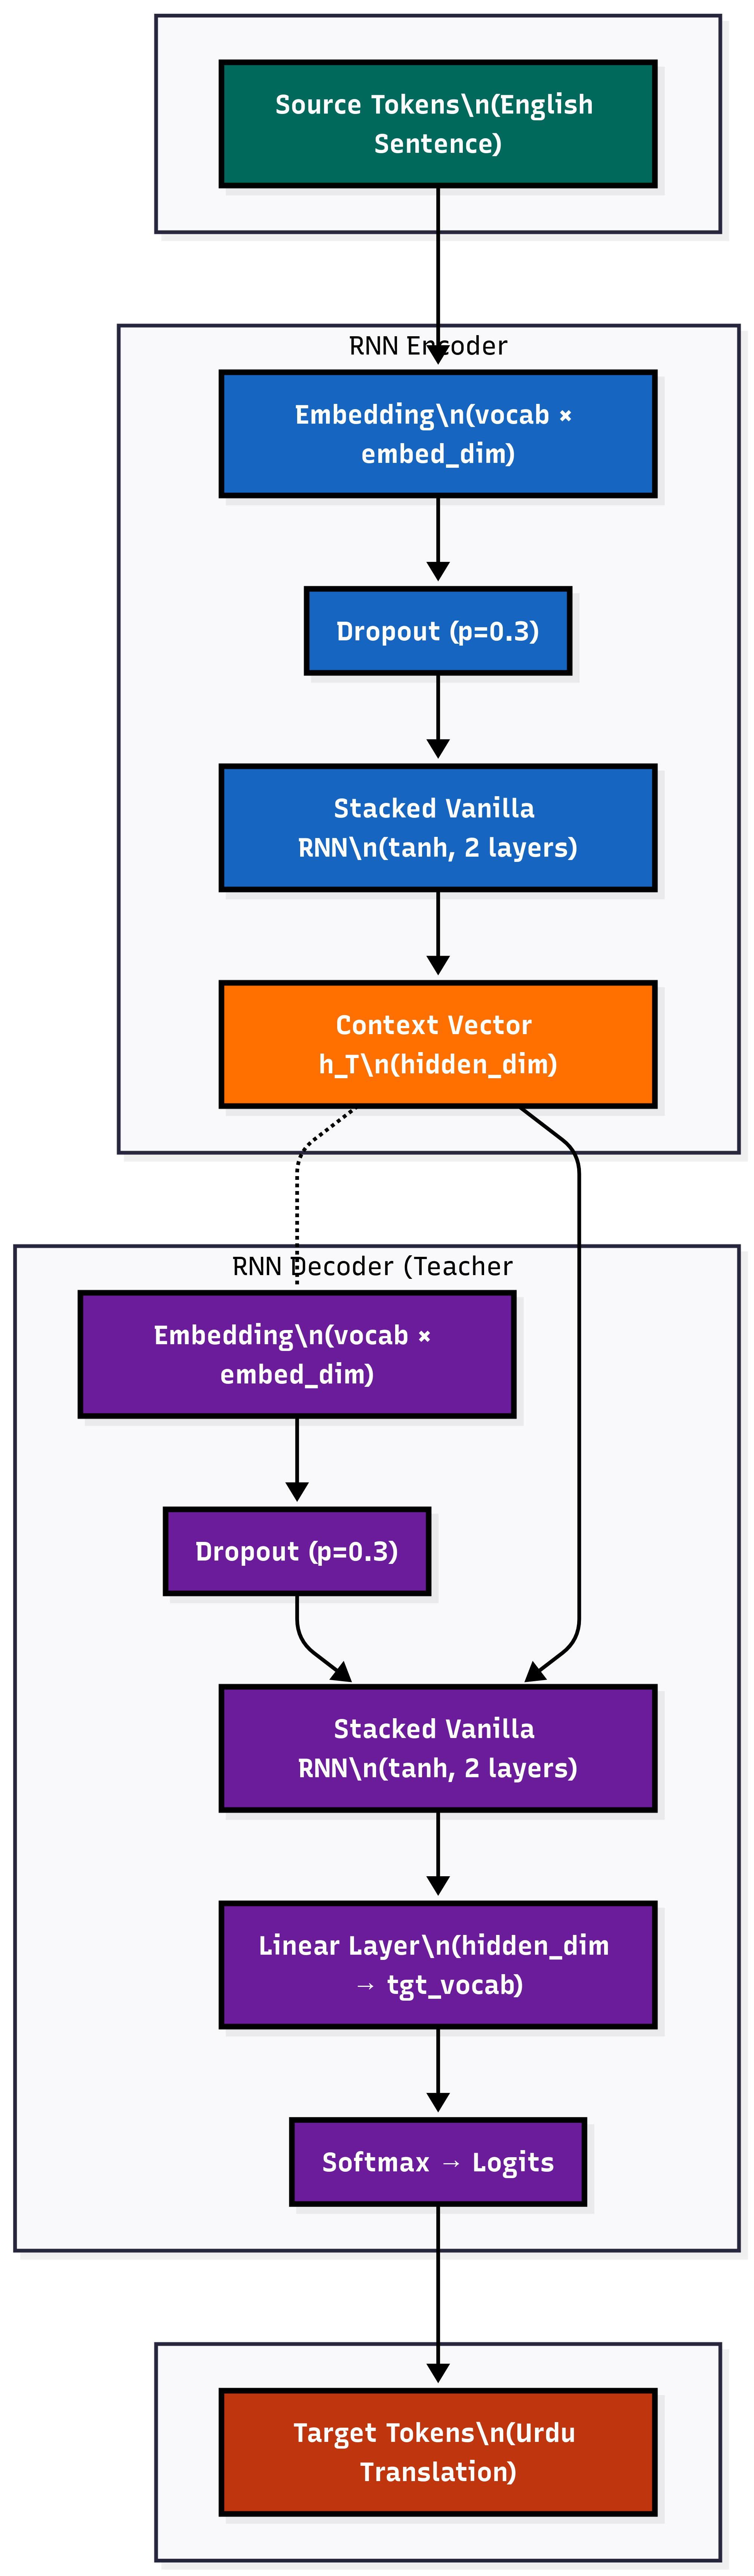
\includegraphics[width=0.9\textwidth]{images/06a_rnn_encoder_decoder.png}
    \caption{Vanilla RNN Encoder-Decoder Architecture Setup.}
    \label{fig:architecture}
\end{figure}

\begin{figure}[H]
    \centering
    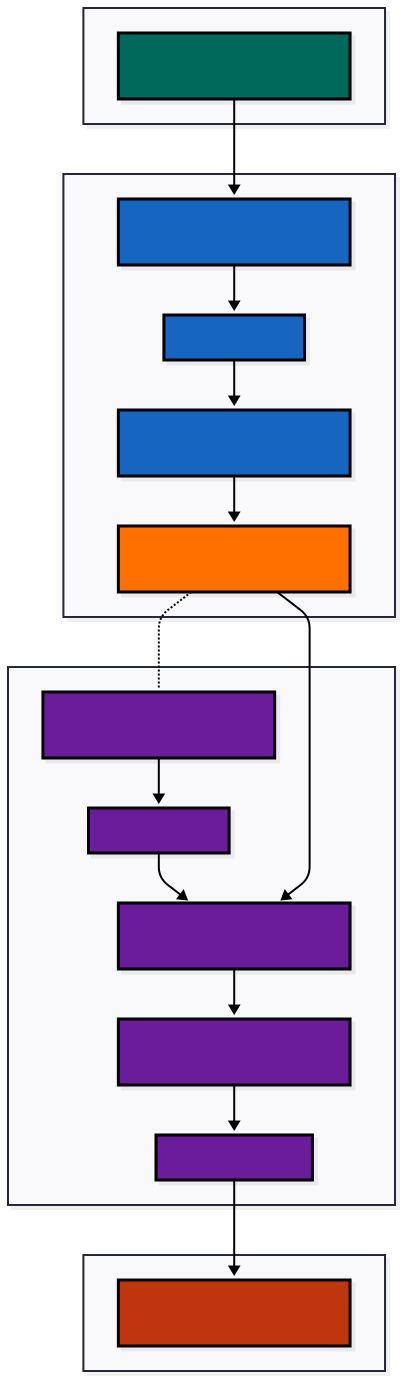
\includegraphics[width=0.6\textwidth]{images/06b_context_vector.svg}
    \caption{Visual representation of the Context Vector mapping.}
    \label{fig:context_vector}
\end{figure}

\section{Training Pipeline and Hyperparameter Tuning}

\subsection{Optimization Strategy}
Exploding gradients are a notorious failure mode for Vanilla RNNs. Consequently, \textbf{Gradient Clipping} with a max norm of 1.0 was universally enforced. We utilized the Adam optimizer coupled with a \texttt{ReduceLROnPlateau} scheduler to dynamically halve the learning rate upon validation loss stagnation.

\begin{figure}[H]
    \centering
    
\includegraphics[width=0.8\textwidth]{outputs/plots/07_training_dynamics.png}
    \caption{Training Dynamics: Loss curves and perplexity over epochs}
    \label{fig:training}
\end{figure}

\subsection{Grid Search Study}
A multidimensional Grid Search was conducted evaluating combinations of embedding dimensionality (128, 256), hidden dimensionality (256, 512), RNN depth (1, 2), learning rates (1e-3, 5e-4), dropout probabilities (0.2, 0.3), and batch sizes (32, 64). 

Table~\ref{tab:hyperparams} justifies the optimal configuration based on optimal Val Loss configurations without exploding to \texttt{NaN}.

\begin{table}[H]
    \centering
    \caption{Optimal Hyperparameter Configuration based on Grid Search}
    \label{tab:hyperparams}
    \begin{tabular}{llc}
        \toprule
        \textbf{Hyperparameter} & \textbf{Searched Range} & \textbf{Optimal Value} \\
        \midrule
        Embedding Size & \{128, 256\} & 128 \\
        Hidden Dimension & \{256, 512\} & 256 \\
        Num RNN Layers & \{1, 2\} & 1 \\
        Learning Rate & \{1e-3, 5e-4\} & 1e-3 \\
        Dropout (p) & \{0.2, 0.3\} & 0.2 \\
        Batch Size & \{32, 64\} & 64 \\
        \textbf{Total Parameters} & -- & \textbf{2,262,910} \\
        \bottomrule
    \end{tabular}
\end{table}

\begin{figure}[H]
    \centering
    
\includegraphics[width=0.8\textwidth]{outputs/plots/08_hyperparameter_search.png}
    \caption{Hyperparameter Search Evaluation Metrics}
    \label{fig:gridsearch}
\end{figure}

Following Grid Search, the model converged within 2 epochs rapidly reaching a best validation loss of 4.4472 and Perplexity of 85.39.

\section{Evaluation and Decoding}

We compared two distinct auto-regressive decoding inferences: \textbf{Greedy Search} ($argmax$ per step) and \textbf{Beam Search} ($k=4$). Results are recorded in Table~\ref{tab:bleu}. 

\begin{table}[H]
    \centering
    \caption{Test Set BLEU Score Evaluation}
    \label{tab:bleu}
    \begin{tabular}{lcccc}
        \toprule
        \textbf{Decoding Method} & \textbf{BLEU-1} & \textbf{BLEU-2} & \textbf{BLEU-3} & \textbf{BLEU-4} \\
        \midrule
        Greedy Decoding & 9.746 & 3.755 & 1.202 & 0.399 \\
        Beam Search ($k=4$) & 4.377 & 1.765 & 0.551 & 0.183 \\
        \bottomrule
    \end{tabular}
\end{table}

\begin{figure}[H]
    \centering
    
\includegraphics[width=0.8\textwidth]{outputs/plots/09_bleu_evaluation.png}
    \caption{BLEU Score Evaluation: Greedy vs. Beam Search}
    \label{fig:bleu}
\end{figure}

Interestingly, Greedy Decoding severely outperformed Beam Search. In Vanilla RNNs lacking explicit coverage models, Beam Search frequently biases toward pathologically short, high-probability repetition loops. 

\section{Error Analysis and Research Findings}

A manual, qualitative error anatomy was conducted over translated sentences evaluating failure patterns spanning repetitions, hallucinations, and under-generation.

\subsection{Qualitative Limitations of Vanilla RNNs}
\begin{enumerate}
    \item \textbf{Information Bottleneck:} The entire English source token sequence must fundamentally map down into a highly restricted vector dimensionality. Detail is systematically lost on longer sequences (e.g., length $> 15$).
    \item \textbf{Reordering Collapse (SVO $\to$ SOV):} Translating the English Subject-Verb-Object into the Urdu Subject-Object-Verb requires holding the initial subject and verb in memory until the object has been subsequently decoded. Regular RNN architectures lack the memory horizons to delay output mapping, usually causing grammatical corruption. 
    \item \textbf{Vanishing Gradients:} Long dependencies suffer gradient decay via the recurrent \texttt{tanh} derivative multiplication.
    \item \textbf{Out-of-Distribution (OOD) Degradation:} Evaluating sentences at the 90th percentile of length and OOV-density resulted in an OOD BLEU-4 of 0.088 vs. an In-Distribution BLEU-4 of 0.207 (a catastrophic $+0.119$ drop). 
\end{enumerate}

\begin{figure}[H]
    \centering
    
\includegraphics[width=0.8\textwidth]{outputs/plots/10_error_analysis.png}
    \caption{Error Taxonomy and OOD Analysis}
    \label{fig:errors}
\end{figure}

\subsection{Future Improvements}
Future iterations could drastically resolve these issues by substituting the Vanilla RNN explicitly for LSTMs or GRUs, adding Bi-Directional encoding to capture context simultaneously, and integrating Global Attention (e.g., Luong or Bahdanau) to distribute the translation burden per decoding step rather than relying entirely on a stationary context bottleneck.

\end{document}
